%%
%% Author: dariochinelli
%% 2021-03-23
%%

\section{Teoria quanto-meccanica di Shrodinger}
Con questa teoria è possibile esprimere l'equazione che controlla l'evoluzione di una funzione d'onda.
Essa è una funzione delle coordinate spaziali e del tempo, avente il significato di un'ampiezza di probabilità.
Sostanzialmente amplia il concetto dell'ipotesi di De Broglie.
Questa è l'espressione del moto di una particella libera con momento costante
\begin{equation}
\begin{split}
& \lambda = \frac{ h}{p } \\
& \Psi(x,t) = \sin \biggl[ 2 \pi \biggl( \frac{x}{\lambda} - \nu t \biggr) \biggr]
\end{split}
\end{equation}
Tuttavia se voglio considerare una particella con momento non costante, quindi su cui agisce una forza, essa è troppo semplice e occorre cercare un'equazione più complicata, che soddisfi le seguenti condizioni:
\begin{enumerate}
\item consistente con $\lambda = \frac{ h}{p }$ e $\nu = \frac{ E}{ h}$
\item consistente con $E = \frac{p^2}{2m} + V$
\item Lineare: ogni combinazione lineare di soluzioni deve essere anch'essa soluzione.
\item condizione di particella libera: $V(x,t) = V_0 = cost. \Rightarrow F=-\frac{ \partial V(x,t)}{ \partial x} = 0$
\end{enumerate}
Nel caso di particella libera la soluzione dovrà appartenere al campo complesso e avrà forma
\begin{equation}
\begin{split}
& \Psi (x,t) = \cos(kx-\omega t) + i \sin(kx - \omega t) \\
& \mbox{con} \quad k = \frac{2\pi}{\lambda}
\end{split}
\end{equation}


\paragraph{Equazione di Schrodinger} Nel 1925 Schrodinger postulò l'equazione per una particella quantistica:
\begin{equation}
- \frac{\hbar^2}{2m} \frac{\partial^2 \Psi(x,t)}{\partial x^2} + V(x,t) \Psi(x,t) = i \hbar \frac{\partial \Psi(x,t)}{\partial t}
\label{eq_schrodinger}
\end{equation}
Essendo $\Psi$ una funzione complessa cade l'idea di immaginarsi cosa ondeggi nel moto della particella.


\paragraph{Postulato di Born (1926)} Si può definire $P(x,t)$, che esprime la probabilità di localizzare una particella, come:
\begin{equation}
\begin{split}
P(x,t) dx & = \Psi^{\ast}(x,t)\Psi(x,t) dx \\
P(x,t) & = \Psi^{\ast}(x,t)\Psi(x,t) = |\Psi(x,t)|^2
\end{split}
\end{equation}


\subsection{Derivazione della TISE}
L'equazione di Shrodinger dipende dalle due variabili $x$ e $t$ ma si può risolvere mediante la \underline{tecnica di separazione delle variabili}, a patto che il potenziale non dipenda dal tempo ma solo da $x$
\begin{equation}
\begin{split}
& \Psi(x,t) = \psi(x)\varphi(t) \\
& -\frac{\hbar^2}{2m} \frac{\partial^2 \psi(x)}{\partial x^2}+ V(x)\psi(x) = E\psi(x)
\end{split}
\end{equation}
ottengo l'Equazione di Schrodinger indipendente dal tempo, si noti che non è esplicitamente un valore complesso.
E si trova, separatamente, la seguente soluzione per la parte temporale $\varphi$
\begin{equation}
\begin{split}
& \frac{d \varphi(t)}{dt} = - \frac{i E}{\hbar} \varphi(t) \\
& \varphi(t) = e^{-i \frac{E}{\hbar} t}
\label{eq_sch_temp}
\end{split}
\end{equation}

Come si arriva alla equazione di Schrodinger indipendente dal tempo
\begin{equation}
\begin{split}
& \frac{ p^2}{2m } + V = E \\
& p = \frac{ h}{\lambda } = \hbar k \quad \mbox{con } k = \frac{ 2\pi}{\lambda } \\
& \frac{ \hbar^2 k^2}{2m } + V = E \\
& k^2 \frac{ 2m}{\hbar^2 } (E-V)
\end{split}
\end{equation}
la funzione $\psi$ per una particella libera e le sue derivate sono
\begin{equation}
\begin{split}
\psi(x) & = \sin\frac{2\pi x}{\lambda } = \sin kx \\
\frac{ d \psi(x)}{dx } & = k \cos kx \\
\frac{ d^2 \psi(x)}{dx^2 } & = -k^2 \sin kx = -k^2 \psi(x) \\
\frac{ d^2 \psi(x)}{dx^2 } & = -\frac{ 2m}{\hbar^2 } (E-V) \psi(x) \\
-\frac{\hbar^2}{2m} \frac{\partial^2 \psi(x)}{\partial x^2} & + V(x)\psi(x) = E\psi(x)
\end{split}
\end{equation}
si ottiene così la funzione d'onda indipendente dal tempo, per ricavare il caso più generale si veda il corso di MQ.
Per postulato si afferma che questa equazione sia valida anche nel caso di una particella soggetta ad una forza.


\subsection{Particella libera} Soluzione per l'equazione di Schrodinger nel caso di una particella libera
\begin{equation}
\mbox{particella libera } \quad\Rightarrow\quad V(x) = costante \quad\Leftrightarrow\quad  F = - \frac{ dV(x)}{dx } = 0
\end{equation}
poiché il potenziale è una costante posso sceglierlo nullo, ovvero $V(x) = 0$.
L'equazione di Schrodinger indipendente dal tempo è
\begin{equation}
- \frac{ \hbar^2}{2m } \frac{ d^2 \psi(x)}{dx^2 } = E \psi(x)
\end{equation}
La soluzione generale dipendente dal tempo si ricava essere il prodotto tra la $\psi(x)$ soluzione all'equazione spaziale e la $\phi(t)$ soluzione all'equazione temporale \ref{eq_sch_temp} , ovvero
\begin{equation}
\Psi(x, t) = \psi(x) e^{ -\frac{ i E t}{\hbar } }
\label{psi_1}
\end{equation}
ed è anche vero che possiamo esprimere la funzione d'onda totale come 
\begin{equation}
\begin{split}
\Psi (x,t) & = \cos(kx-\omega t) + i \sin(kx - \omega t) \\
& = e^{ i (kx - \omega t) } = e^{ ikx } e^{ -i \omega t }
\end{split}
\label{psi_2}
\end{equation}
confrontando le due forme \ref{psi_1} e \ref{psi_2} di $\Psi(x, t)$ emerge subito l'equazione
\begin{equation}
\psi(x) = e^{ ikx }
\end{equation}
ricordando le forme di $k$ e $\omega$
\begin{equation}
k = \frac{ p}{\hbar } = \frac{ \sqrt{2mE}}{\hbar } \quad \quad \omega=\frac{ E}{\hbar }
\end{equation}
In effetti le soluzioni all'TISE (Time Indipendent Schrodinger Equation) sono due
\begin{equation}
\begin{split}
& \psi(x) = e^{ ikx } \\
& \psi(x) = e^{ - ikx }
\end{split}
\end{equation}
e quindi anche una combinazione lineare delle due deve essere una soluzione alla TISE
\begin{equation}
\psi(x) = A e^{ ikx } + B e^{- ikx }
\end{equation}
Se ho la condizione per cui $|A| = |B|$ si realizza il caso di onda stazionaria, ovvero ho due onde "viaggianti" in direzioni opposte.
Notare inoltre che in tale condizione la particella potrà trovarsi ovunque in $x$ e 
\begin{equation}
\begin{split}
\psi^{\ast}(x)\psi (x)= A^{\ast} A \quad\Rightarrow\quad  \Delta x = \infty \quad \Delta p = 0
\end{split}
\end{equation}
la notazione di Schrodinger deve necessariamente essere consistente con il Principio di Indeterminazione di Heisemberg.


\paragraph{Esempio: Buca infinita di potenziale}
Considero il caso 1-dimensionale, in cui la particella è confinata in una regione di spazio in cui il potenziale è nullo e fuori dal quale è infinito.
\begin{figure}[h]
\centering
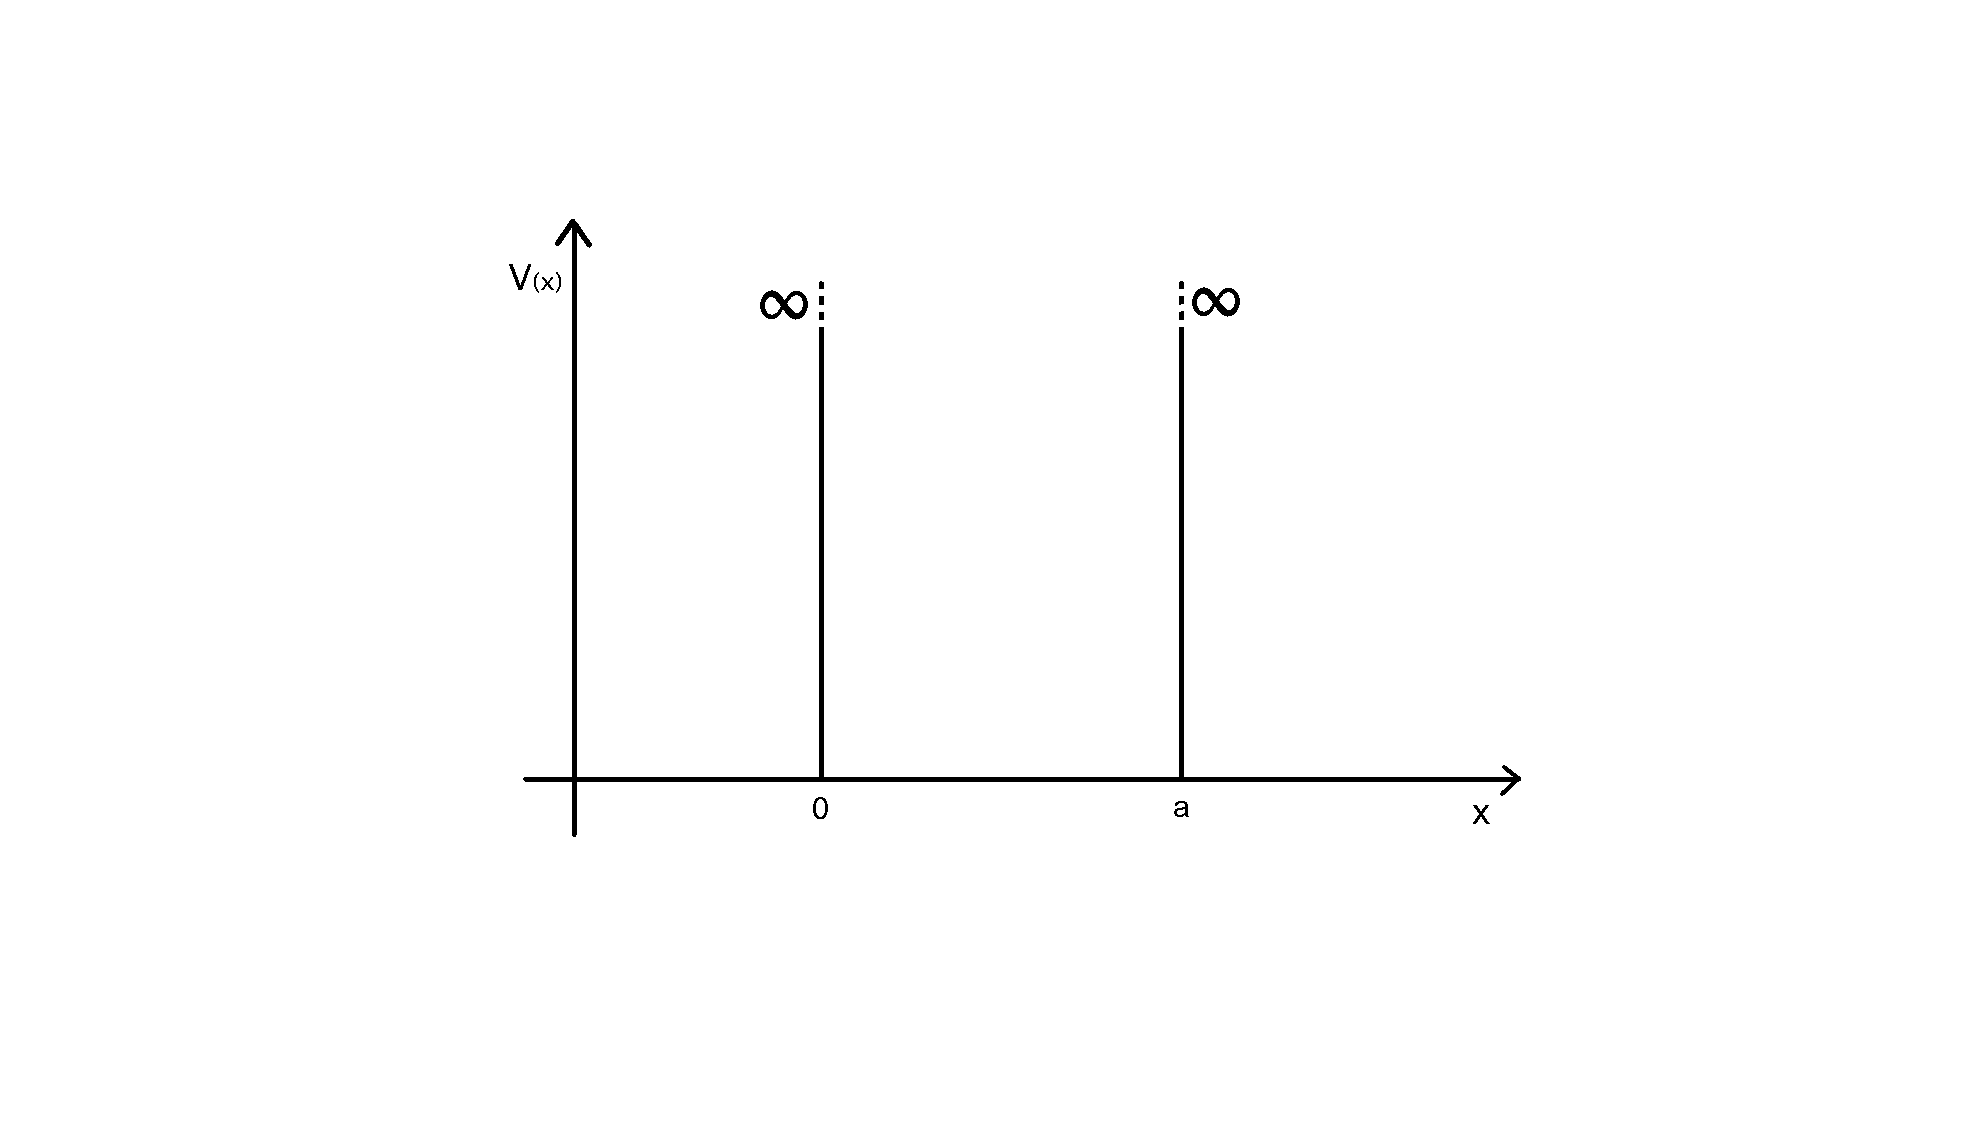
\includegraphics[scale=0.4]{/pot_inf}
\end{figure}
% potenziale buca infiinta
\begin{equation}
V(x) = 
\begin{cases}
	\infty \quad\quad x>a \vee x<0 & \quad\quad \mbox{regione \rm{I}} \\
	0 \quad\quad\quad 0 < x < a & \quad\quad \mbox{regione \rm{II}}
\end{cases}
\end{equation}
nella regione \rm{I} del potenziale la funzione d'onda dovrà essere nulla per cui $\psi(x)  = 0$, invece la funzione d'onda nella regione \rm{II} sarà $\psi (x) = A e^{i k x} + B e^{- i k x} $, quindi la particella è libera di muoversi avanti e indietro nell'intervallo $[0, a]$.
La funzione d'onda deve però essere stazionaria, non "viaggiante", poiché ha dei nodi fissi in corrispondenza degli estremi.
Quindi imponendo la condizione di annullamento di $\psi$ agli estremi ci permette di ricavare per l'estremo $x=0$
\begin{equation}
\begin{split}
& \psi(0) = A + B = 0 \quad\Rightarrow\quad  B = - A \\
& \Psi (x) = A ( e^{i k x} - e^{- i k x} ) = 2 i A \sin(k x) = c \sin(k x) \\
& \Rightarrow\quad c = 2 i A
\end{split}
\end{equation}
e per $x=a$
\begin{equation}
\begin{split}
& \psi(a) = c \sin(k a) = 0 \\
& \Rightarrow\quad c = 0 \quad \mbox{caso banale} \quad\Rightarrow\quad c\not= 0 \\
& \Rightarrow\quad \sin(k a) = 0 \quad\Leftrightarrow\quad ka = n \pi \quad \mbox{ con } n \in Z \\
& k = \frac{ n\pi}{a } \quad\Rightarrow\quad  p = \hbar k = \frac{ n \pi \hbar}{a }
\end{split}
\end{equation}
si ritrova la quantizzazione del momento $p$.
\begin{equation}
E = \frac{p^2}{2m} = \frac{\hbar^2 k^2}{2m} = \frac{\hbar^2 n^2 \pi^2 }{2 m a^2} \quad \mbox{ con } n \in Z
\end{equation}
A differenza della meccanica classica, in meccanica quantistica l'energia della particella (confinata) è quantizzata: può quindi assumere solo certi valori di energia \textit{permessi}.
\begin{equation}
\begin{split}
E & = \frac{ \hbar^2 \pi^2 n^2}{2ma^2 } \\
E_1 & = \frac{ \hbar^2 \pi^2}{2ma^2 } \\
E_2 & = 4 \frac{ \hbar^2 \pi^2}{2ma^2 } = 4 E_1 \\
E_3 & = 9 \frac{ \hbar^2 \pi^2}{2ma^2 } = 9 E_1
\end{split}
\end{equation}
Allora le funzioni d'onda per la particella corrispondenti ai diversi valori di $k$ sono
\begin{equation}
\psi_n(x) = c \sin\Bigl(  \frac{ n\pi x}{a }  \Bigr)
\end{equation}
sono le funzioni dell'ampiezza delle onde stazionarie all'interno della buca infinita di potenziale.
Il minimo dell'energia non è zero, bensì $E_1 = \frac{ \hbar^2 \pi^2}{2ma^2}$
è da notare che è una diretta conseguenza del principio di indeterminazione. 


\paragraph{Esempio: Particella in una scatola 3-D}
Il momento $p$ lungo le tre dimensioni sarà dipendente da tre numeri quantici $n_1,n_2,n_3$ e dalle tre dimensioni della scatola $a,b,c$, per cui
\begin{equation}
\begin{split}
p_x = \frac{\pi \hbar n_x}{a} \\
p_y = \frac{\pi \hbar n_y}{b} \\
p_z = \frac{\pi \hbar n_z}{c}
\end{split}
\end{equation}
Per cui l'energia risulta
\begin{equation}
E = \frac{p^2}{2m} = \frac{1}{2m} ( p_x^2 + p_y^2 + p_z^2 )= \frac{\pi^2 \hbar^2}{2m} \Bigl(  \frac{n_x^2}{a^2} + \frac{n_y^2}{b^2} + \frac{n_z^2}{c^2}  \Bigr)
\end{equation}
e l'equazione d'onda diventa
\begin{equation}
\psi(x) = c \sin \frac{n_1 \pi x}{a} \sin \frac{n_2 \pi x}{b} \sin \frac{n_3 \pi x}{c}
\end{equation}
Si ha una scatola cubica se $a=b=c$ per cui l'energia diventa
\begin{equation}
\begin{split}
E & = \frac{\pi^2 \hbar^2}{2 m a^2} r^2 \\ 
r^2 & = n_1^2 + n_2^2 + n_3^2
\end{split}
\end{equation}
Tutti gli stati energetici corrispondenti a diversi valori per $n_1^2, n_2^2, n_3^2$ che portano ad uno stesso valore di $r^2$ hanno la stessa energia, ma non hanno la stessa funzione d'onda.
Il fenomeno è detto di \textit{degenerazione}.
Per valori piccoli di $a$ i livelli energetici sono molto distanti fra loro, se aumento le dimensioni della scatola e $a$ è grande i livelli energetici saranno molto ravvicinati fino a formare quasi un continuo di stati.


\subsection{Densità di livelli energetici} 
Calcoliamo il numero di livelli energetici nel range $dE$ per una particella in una scatola cubica.
Nello spazio degli $n$, che è definito dalla terna $(n_x, n_y, n_z)$, ogni punto $P$ rappresenta un livello di energia possibile per la particella nella scatola cubica.
Tutti i punti che giacciono su una superficie di raggio $r$ hanno la stessa energia.
\begin{equation}
r^2 =  n_1^2 + n_2^2 + n_3^2
\end{equation}
% grafico ottante di sfera
\begin{figure}[h]
\centering
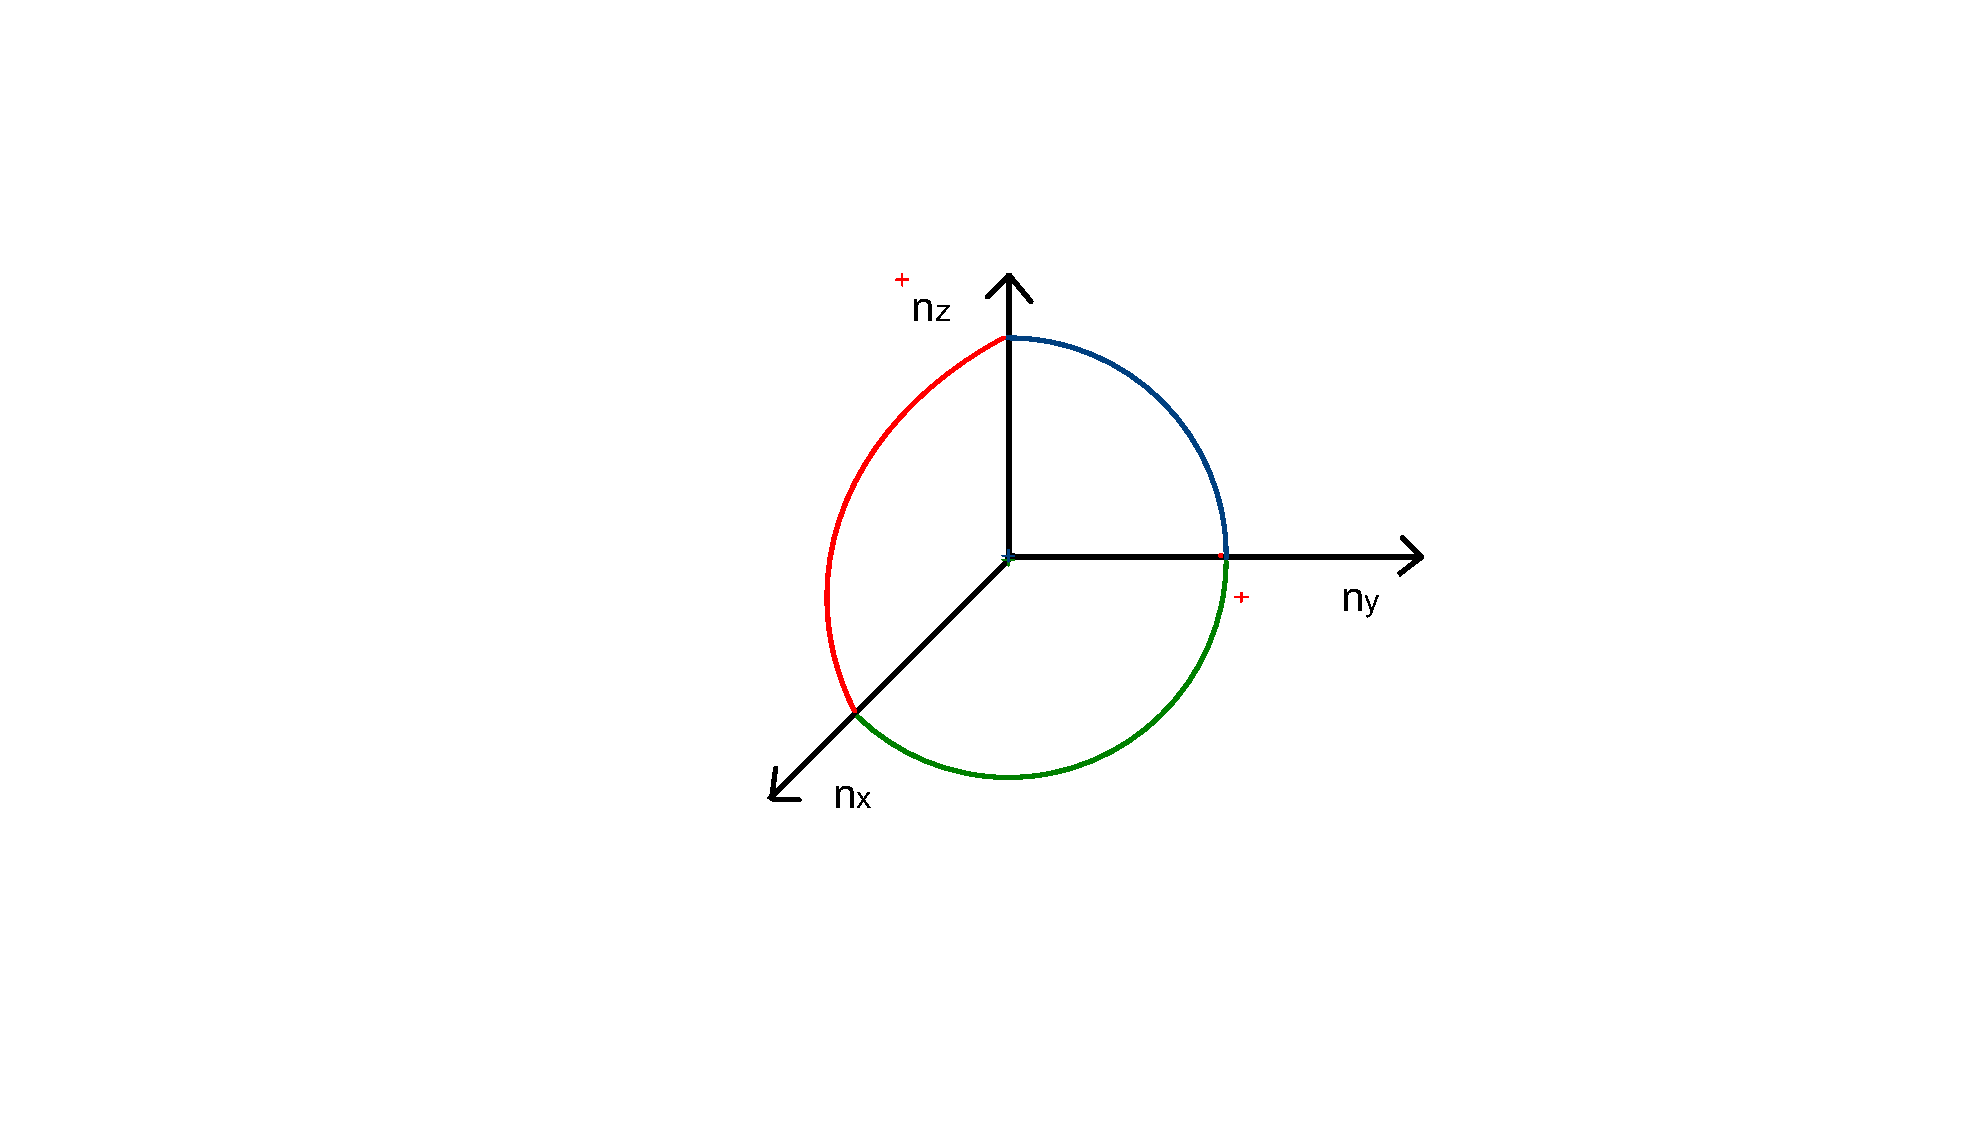
\includegraphics[scale=0.5]{/spazio_nodi}
\end{figure}
Per contare il numero di stati $N(E)$ che sono contenuti in un ottante di sfera calcoliamo il volume $(V=a^3)$ della sfera di raggio $r$ e moltiplichiamo per $\frac{1}{8}$
\begin{equation}
N(E) = \frac{1}{8} \Bigl( \frac{4}{3} \pi r^3 \Bigr) = \frac{\pi}{6} a^3 \Bigl( \frac{2 m E}{\pi^2 \hbar^2} \Bigr) ^{\frac{3}{2}} = 
\frac{8 \pi V}{3 h^3} (2 m^3) ^{\frac{1}{2}} E^{\frac{3}{2}}
\end{equation}
differenziando la relazione precedente si trova
\begin{equation}
dN(E) = \frac{4 \pi V (2 m^3)^{\frac{1}{2}} }{\hbar^3}  E^{\frac{1}{2}} dE
\end{equation}
Si introduce una \textit{funzione densità degli stati} $g(E)$ che definisce il numero di stati di energia possibile nell'intervallo $dE$, definita come
\begin{equation}
g(E) = \frac{ dN}{dE } = \frac{ 4\pi V (2m^3)^{\frac{ 1}{2 }}}{h^3 } E^{ \frac{ 1}{2 } }
\end{equation}
% grafico andamento g
\begin{figure}[h]
\centering
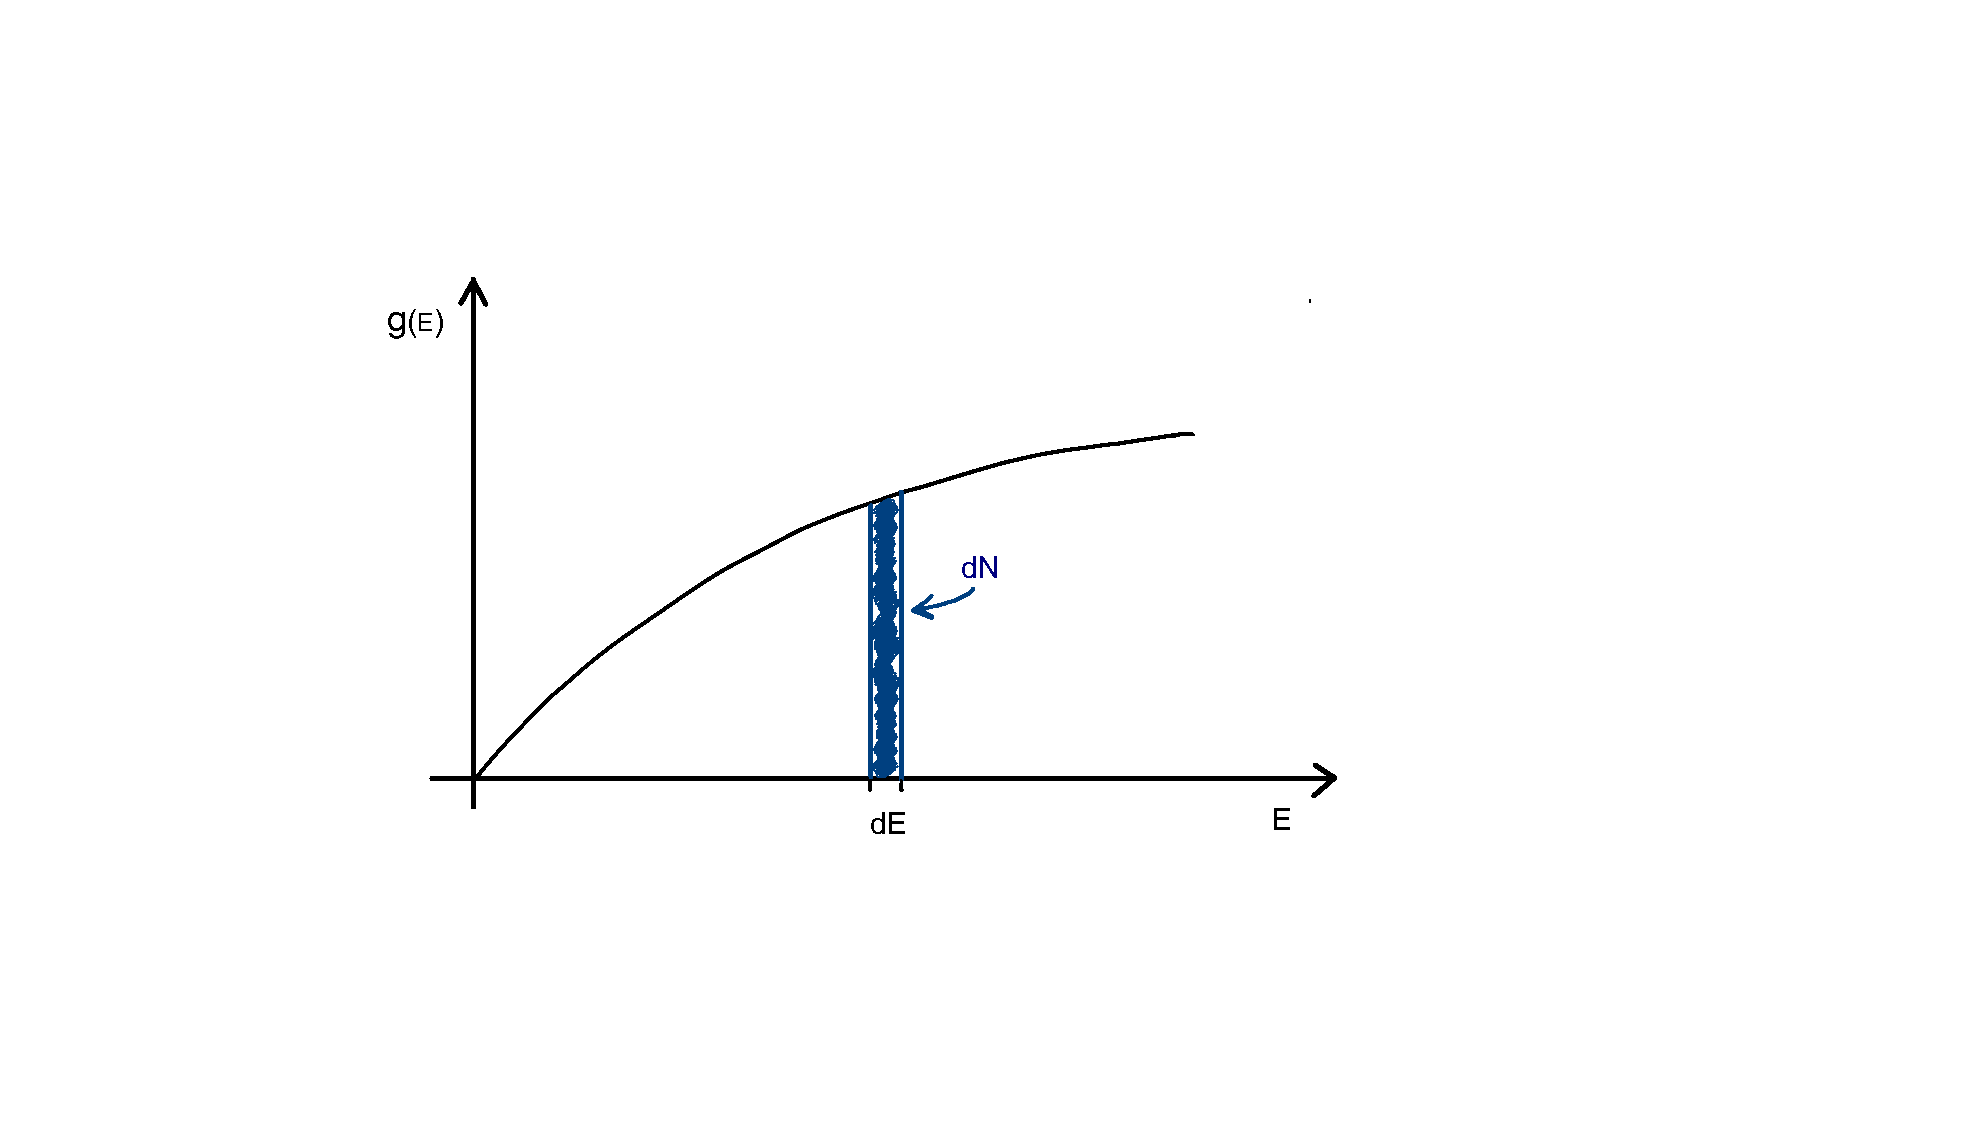
\includegraphics[scale=0.5]{/andamento_g}
\end{figure}
Posso allora definire una \textit{funzione densità degli stati} $g(p)$ dipendente dal momento $p$
\begin{equation}
\begin{split}
& dN = g(p)dp = g(E)dE \\
& \frac{ dN}{dp } = g(p) = g(E) \frac{ dE}{dp } = \frac{ 4\pi V}{h^3 } p^2
\end{split}
\end{equation}

\paragraph{Considero dei fotoni}
\begin{equation}
\begin{split}
& p = \frac{ h }{\lambda } \quad\quad \nu = \frac{ c}{\lambda } \\
& p = \frac{ h\nu}{c }
\end{split}
\end{equation}
Posso allora definire una \textit{funzione densità degli stati} $g(\nu)$ in funzione della frequenza $\nu$
\begin{equation}
\begin{split}
& g(\nu)d\nu = g(p)dp \\
& g(\nu) = g(p)\frac{ dp}{d\nu } = 2 \cdot \frac{ 4\pi V}{c^3 } \nu^2
\end{split}
\end{equation}
dove aggiungo un fattore $2$ poiché sto considerando dei fotoni, delle particelle con $spin=\frac{ 1}{2 }$, che hanno due possibili stati di polarizzazione.
Ottengo così alla relazione per il numero di modi delle frequenze permesse per le onde elettromagnetiche stazionarie nella cavità di corpo nero.
Il tipo di approccio di questi calcoli è simile a quanto visto contando le onde stazionarie come visto nel capitolo sul corpo nero.




